% !TEX root = ../thesis.tex
\chapter{Evaluation} \label{evaluation}
Whole prediction is made 10 times. The final result is arithmetic mean from this prediction which is ten times run to random deviation until is removed.
Our prediction script is finally written in Matlab Live script with predefined constants based on Megaplay s.r.o data,
    but for modeling and dynamic prediction are used Live scripts Controls so in the script we are able to easily set all constant to model for simulate different situations.
    Let see the function of our prepared model.This precalculated data entered calculation loop.
Next loop read the value of predefined number of customers in each period and simulated the virtual customer bavior in order process in the next steps:
We can see model situation in~\ref{apendixc} and that results is described in the final summary~\ref{summary} as results from previous models from section~\ref{sec:baseline}.
Then Matlab's function $predint$ was used to return income prediction results for year 2020 used fitted model in section~\ref{sec:baseline}.
to calculate aberration for each month from plotted results as it seen on figure~\ref{predict}.
\begin{figure}[h!]
    \begin{center}
        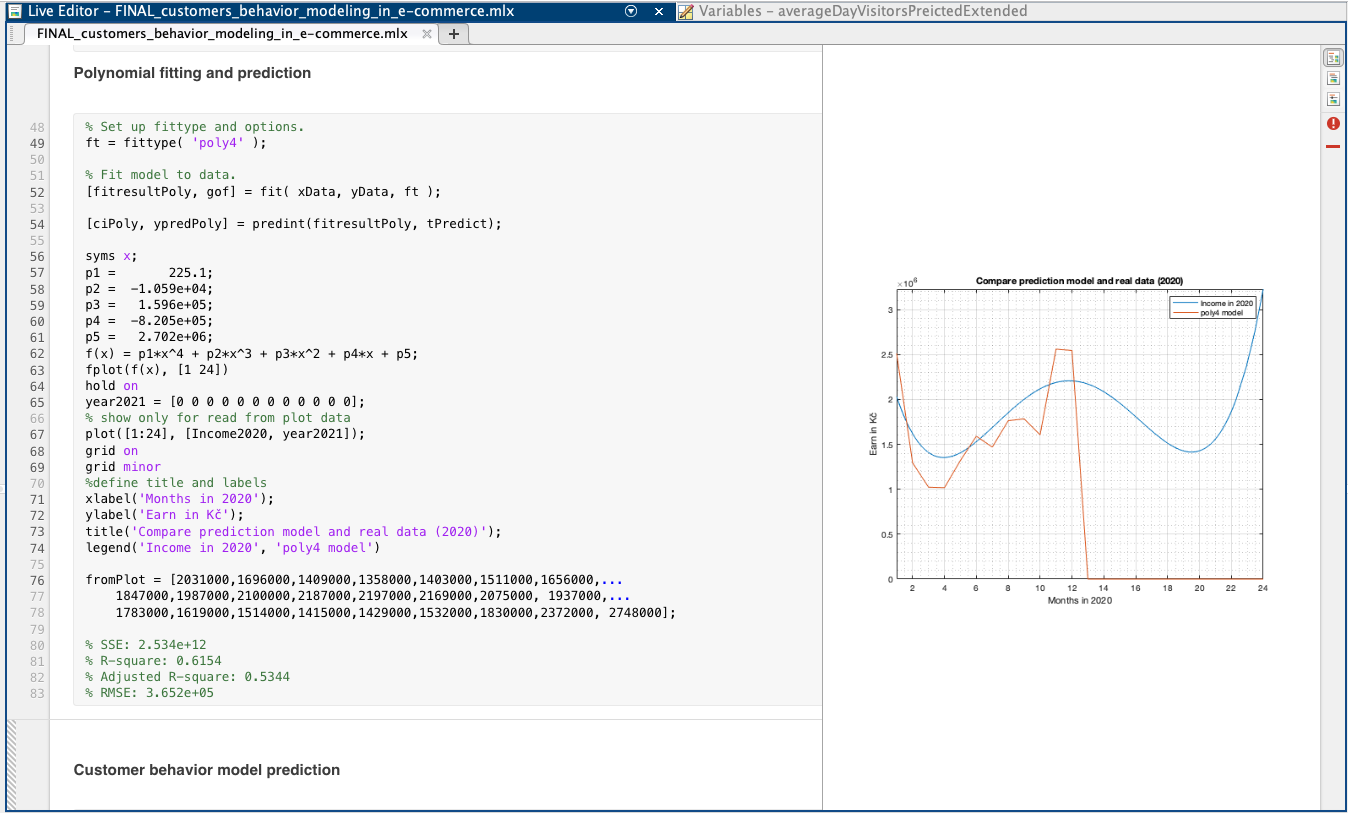
\includegraphics[width=80mm]{predict.png}
    \end{center}
    \caption{Predict income data in live script~\cite{luarn}}
    \label{predict}
\end{figure}\\
Fitted and prepared models from section~\ref{sec:baseline} was compared with real data
Experiment was simulated in Matlab, where internal predefined function was used.
See more in section~\ref{subsec:libraries}.
Let use Matlab Curve fitting tool to solve our linear and polynomial models as you can see on figure 2.4, this predefined tool calculate coefficient for and then the prediction in Matlab Live script was done as we see on figure ?? These two models was fitted on income data from years 2018 and 2019 and used in Experi- ment section 2.2.
\begin{figure}[h!]
    \begin{center}
        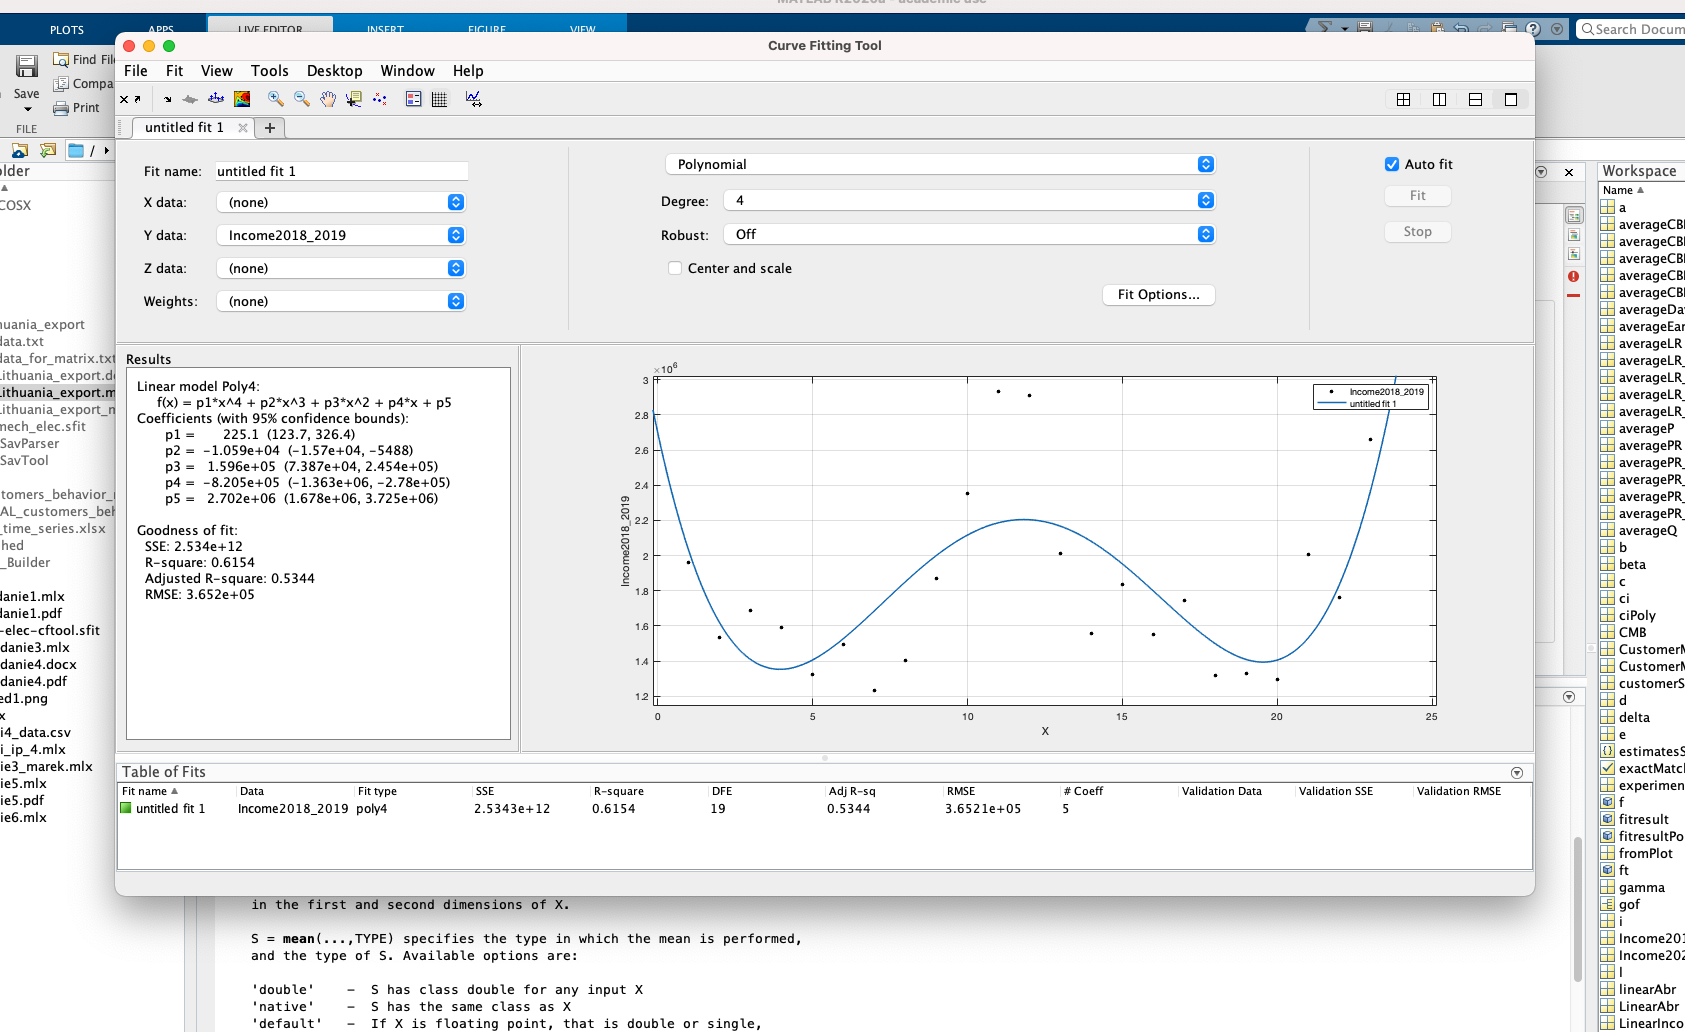
\includegraphics[width=90mm]{cftool.png}
    \end{center}
    \caption{Fitting the data with cftool~\cite{luarn}}
    \label{cftool}
\end{figure}\\



\section{Used software, libraries and predefined functions} \label{subsec:libraries}
\textbf{Matlab 2020a}\\
MATLAB (matrix laboratory) is a fourth-generation high-level programming language and interactive environment for numerical
computation, visualization and programming developed by MathWorks.\\
\\
\textbf{Matlab LiveScript}~\cite{livescript}\\
MATLAB live scripts and live functions are interactive documents that combine MATLAB code with formatted text, equations,
and images in a single environment called the Live Editor.
In addition, live scripts store and display output alongside the code that creates it.\\
Use live scripts and functions to:\\
\begin{itemize}
    \item Visually explore and analyze problems
    \item Share richly formatted, executable narratives
    \item Create interactive lectures for teaching
\end{itemize}\\
\\
\textbf{Matlab Curve Fitting Tool}\\
The Curve Fitting Toolbox provides a collection of GUIs and M-files.
With the toolbox we are able to data preprocessing such as sectioning and smoothing, parametric and nonparametric data fitting,
and also fit statistics which assist us in determining the goodness of fit,analysis capabilities such as extrapolation, differentiation, and integration.
A graphical environment allows you to explore and analyze data sets and fits visually and numerically.\\
\textbf{hhmgenerate}~\cite{hhmgenerate}\\
The function $hmmgenerate$ begins with the model in state 1 at step 0, prior to the first emission.
The model then makes a transition to state $i_1$, with probability $T_{1i_1}$, and generates an emission $a_k_1$ with probability $E_{i_1k_11}$.
$hmmgenerate$ returns $i_1$ as the first entry of states, and $a_k_1$ as the first entry of seq.
$[seq,states] = hmmgenerate(len,TRANS,EMIS)$ takes a known Markov model, specified by transition probability matrix $TRANS$ and emission probability matrix $EMIS$,
and uses it to generate:\\
\begin{itemize}
    \item A random sequence seq of emission symbols
    \item A random sequence states of states
\end{itemize}
The length of both $seq$ and $states$ is $len$.
$TRANS(i,j)$ is the probability of transition from state $i$ to state $j$.
$EMIS(k,l)$ is the probability that symbol $l$ is emitted from state $k$.\\
\\
\textbf{hhmviterbi}~\cite{hhmviterbi}\\
The function $hmmviterbi$ begins with the model in state 1 at step 0, prior to the first emission.
hmmviterbi computes the most likely path based on the fact that the model begins in state 1.
$STATES = hmmviterbi(seq,TRANS,EMIS)$ given a $sequence, seq$, calculates the most likely path through the hidden Markov model
specified by transition probability matrix, $TRANS$, and emission probability matrix $EMIS$. $TRANS(i,j)$ is the probability of transition from state $i$ to state $j$.
$EMIS(i,k)$ is the probability that symbol $k$ is emitted from state $i$.\\
\\
\textbf{shopycrm.com}\\
Online CRM application focused on e-commerce stores which provides all store workflows and get precalculated data which we will use for our models to simplify the prediction calculation.
\newpage
\section{Fitting models}
On the figure~\ref{plot} is graphical presentation of data and our linear and polynomial models.
It turned out that the first linear model (blue line), is not directly corresponding the data, but it is copying the trend of the income,
what we should see on figure~\ref{prediction} with predicted data to 2020.
\begin{figure}[h!]
    \begin{center}
        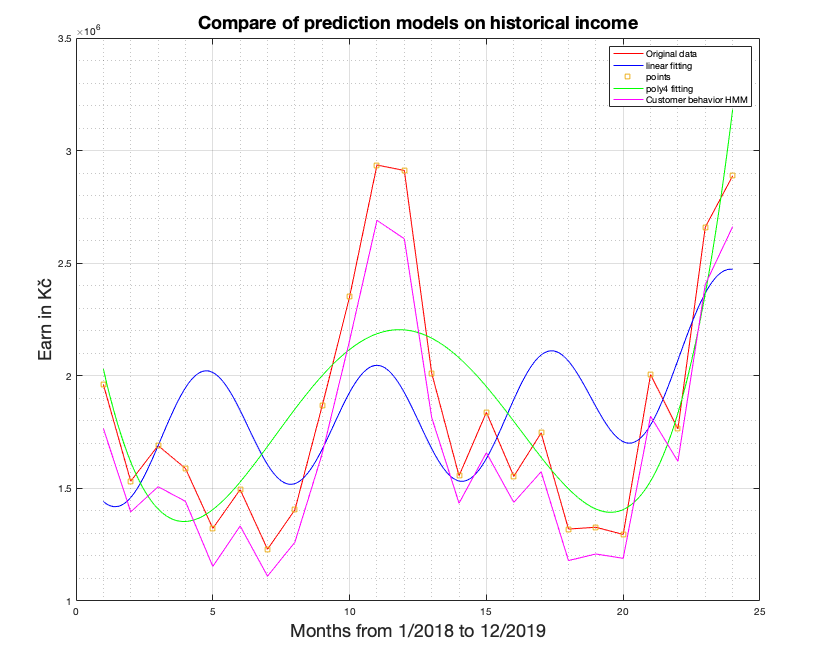
\includegraphics[width=140mm]{plot.png}
    \end{center}
    \caption{Fitting the model on real income from 2018 and 2018}
    \label{plot}
\end{figure}\\
\newpage
\section{Results} \label{compareresults}
\begin{table}[h!]
    \begin{center}
        \begin{tabular}{ | l | c | c | c |}
            \hline
            & \textbf{}$ \textbf{linear model} & \textbf{polynomial model} & \textbf{Customer behavior HMM}\\
            \hline
            \textbf{SSE} & 5.165.10^{12} & 2.534.10^{12} & 1.717.10^{11} \\
            \textbf{R-square} & 0.2162 & 0.6154 & 0.95 \\
            \textbf{RMSE} & 4.959.10^5 & 3.652.10^5 & 1.196.10^5\\
            \hline
        \end{tabular}
    \end{center}
    \caption{Compare results table for models.}
    \label{compare}
\end{table}\\
\begin{table}[h!]
    \begin{center}
        \begin{tabular}{ | l | c | c | c | c | c | c | c |}
            \hline
            {\textbf{Month}} & \textbf{Real income} & \textbf{1st model} & \textbf{(\%)}  & \textbf{2nd model} & \textbf{(\%)} & \textbf{3rd model} & \textbf{(\%)}\\
            \hline
            1/2021 & 2 510 086 & 2 372 333 & 6 & 2 031 000 & 24 & 2 679 419 & 7\\
            2/2021 & 1 293 778 & 2 256 560 & 74 & 1 696 000 & 31 & 1 367 816 & 6\\
            3/2021 & 1 022 762 & 2 340 092 & 129 & 1 409 000 & 38 & 1 092 252 & 7\\
            4/2021 & 1 017 408 & 2 671 671 & 163 & 1 358 000 & 38 & 1 151 301 & 13\\
            5/2021 & 1 320 608 & 3 086 545 & 134 & 1 403 000 & 6 & 1 369 985 & 4\\
            6/2021 & 1 590 878 & 3 359 684 & 111 & 1 511 000 & 5 & 1 632 372 & 3\\
            7/2021 & 1 468 808 & 3 413 621 & 132 & 1 656 000 & 13 & 1 575 324 & 7\\
            8/2021 & 1 762 959 & 3 390 580 & 92 & 1 847 000 & 5 & 1 959 480 & 11\\
            9/2021 & 1 782 582 & 3 522 629 & 98 & 1 987 000 & 11 & 1 950 306 & 9\\
            10/2021 & 1 605 396 & 3 919 220 & 144 & 2 100 000 & 31 & 1 765 984 & 10\\
            11/2021 & 2 559 070 & 4 467 471 & 75 & 2 187 000 & 17 & 2 611 529 & 2\\
            12/2021 & 2 544 271 & 4 936 855 & 94 & 2 197 000 & 16 & 2 610 694 & 3\\
            \hline
        \end{tabular}
    \end{center}
    \caption{Compare results}
    \label{Compare results}
\end{table}\\
In the graphical view we saw that all our models copy the income, but some of them are easier to calculate, this differences you can see described in summary~\ref{summary}.
\begin{figure}[h!]
    \begin{center}
        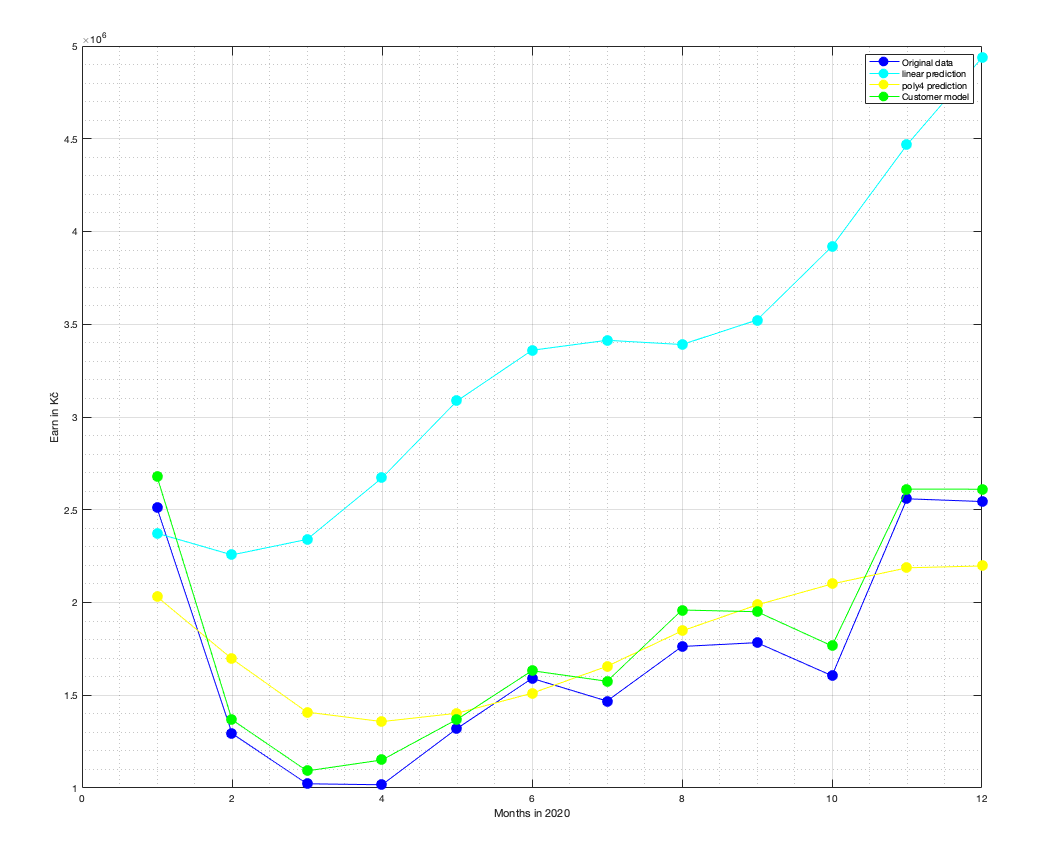
\includegraphics[width=100mm]{prediction.png}
    \end{center}
    \caption{Prediction for year 2020}
    \label{prediction}
\end{figure}\\
\newpage
\begin{table}[h!]
    \begin{center}
        \begin{tabular}{ | l | c | c | c |}
            \hline
            & \textbf{1st model} & \textbf{2nd model} & \textbf{3rd model}\\
            \hline
            1Q (\%) & 69,66 & 30,81 & 6,42\\
            2Q (\%) & 135,83 & 15,00 & 6,50\\
            3Q (\%) & 107,41 & 9,64 & 9,25\\
            4Q (\%) & 104,25 & 21,21 & 4,89\\
            \hline
        \end{tabular}
    \end{center}
    \caption{Quarterly results}
    \label{qResults}
\end{table}
\newpage
